\part{Guide d'installation}

L'installation de \gls{sae} nécessite l'installation de \gls{python} et de \gls{pip}.\\
La version minimale de \gls{python} demandé est \textbf{3.7.*}, les versions \textbf{3.9} et supérieur n'ont pas été
testées.\\
Référer vous à la documentation de votre distribution (ou OS) pour savoir comment les installer.

\section{Depuis les fichiers sources}

Dans toute cette section, nous considérons que le terminal est placé au niveau du dossier du projet.

\begin{minted}{bash}
    cd path/vers/le/dossier/du/projet
\end{minted}

\subsection{Installation des \glsentryplural{paquet}}

Afin de pouvoir utiliser \gls{sae}, certains \glspl{paquet} sont nécessaires.\newline

L'installation des \glspl{paquet} peut être rapidement faite en utilisant le fichier \texttt{requirements.txt} se
trouvant à la racine du projet :

\begin{minted}{bash}
    python3 -m pip install -r requirements.txt
\end{minted}

Les dépendances de chaque \glspl{paquet} s'installeront automatiquement.\newline

En cas d'erreur référez-vous à la documentation du \gls{paquet} concernait ou à la section \nameref{sec:listePackages}.\newline

Copier le dossier \texttt{clearway} sur la cible souhaité (\gls{raspberry}, ou ordinateur, voir section
\nameref{sec:copieVersRaspberry}) et exécuté la commande suivante :

\begin{minted}{bash}
    python3 -m chemin/vers/dossier/clearway
\end{minted}


\subsubsection{Liste des \glsentryplural{paquet}}
\label{sec:listePackages}

Il est aussi possible d'installer individuellement chaque \glspl{paquet} afin d'avoir une installation minimale de \gls{sae}.

\begin{minted}{bash}
    python3 -m pip install <package>
\end{minted}

\begin{itemize}
    \item Nécessaire pour le fonctionnement
          \begin{description}
              \item[transitions] Une implémentation légère et orienté objet de la machine à états en \gls{python} \cite{transition}
              \item[RPi.GPIO] Fournit une classe pour contrôler le GPIO sur une Raspberry Pi \cite{rpi_gpio}.\\
                  Une erreur peut survenir lors de son installation, il peut parfois être nécessaire d'entrer la commande
                  \mintinline{bash}{export CFLAGS=-fcommon} avant afin de pouvoir bien compiler et installer le \gls{paquet}.\\
                  Ce \gls{paquet} est toutefois optionnel si vous choisissez d'utiliser \gls{sae} sans le contrôle des GPIOs
                  (voir section \nameref{sec:executionArg_clearWay})
              \item[imutils] Une série de fonctions de commodité pour rendre les fonctions de traitement d'image de
                  base \cite{imutils}
              \item[numpy] Permet d’effectuer des calculs numériques avec \gls{python} \cite{numpy}
              \item[opencv-python] Bibliothèque open-source pour la vision par ordinateur, l'apprentissage automatique
                  et le traitement des images \cite{opencv}
              \item[toml] Analyse et créer des fichiers \gls{toml} \cite{python_toml}
              \item[Mock.GPIO] Bibliothèque de \glspl{mock} pour la bibliothèque \gls{python} \textit{RPi.GPIO} \cite{mock_gpio}.
          \end{description}

    \item Nécessaire pour les tests
          \begin{description}
              \item[pytest] \Gls{framework} permettant d'écrire facilement des tests petits et lisibles \cite{pytest}
              \item[pytest-cov] Produit un rapport de couverture avec de tests réalisés avec \textit{pytest} \cite{pytest_cov}
              \item[pytest-mock] Fournit un injecteur de \gls{mock} \cite{pytest_mock}
              \item[flake8-pytest-style]
                  Vérifie les problèmes de style communs ou les incohérences \cite{flake8_pytest_style}.
          \end{description}

    \item Génération du \gls{paquet} du \gls{sae} (optionnel)
          \begin{description}
              \item[build] Outil de construction simple qui n'effectue aucune gestion des dépendances. \cite{build}
          \end{description}

    \item Formater et linter (optionnel)
          \begin{description}
              \item[black] Formateur de code \gls{python} \cite{black}
              \item[flake8] Combinaison d'outils pour vérifier la code par rapport au style de codage PEP8
                  \cite{flake8, pep8}
                  \begin{description}
                      \item[flake8-bandit] Tests de sécurité automatisés \cite{flake8_bandit}
                      \item[flake8-import-order] Vérifie l'ordre de vos importations \cite{flake8_import_order}
                      \item[flake8-docstrings] Vérifie la conformité aux conventions des \gls{docstring} \gls{python}
                          \cite{flake8_docstrings}
                      \item[flake8-bugbear] Trouve les probables bogues et problèmes de conception dans le code
                          \cite{flake8_bugbear}
                      \item[flake8-return] Vérifie les valeurs de retour des fonctions dans le code \cite{flake8_return}
                      \item[pep8-naming] Vérifie le code par rapport aux conventions de nommage PEP8 \cite{pep8_naming, pep8}.
                  \end{description}
              \item[mypy]
                  Vérificateur de type statique pour \gls{python}. \cite{mypy}.
          \end{description}
\end{itemize}

\section{Installation avec \glsentryname{pip}}

Il est possible de facilement distribuer \gls{sae} sur plusieurs Raspberry Pi en utilisant \gls{pip}. Pour
cela il est nécessaire d'installer le \gls{paquet} \textit{build} (voir section \nameref{sec:listePackages}).

\begin{minted}{bash}
    python3 -m build
\end{minted}

Cette commande va alors créer un dossier \texttt{dist} et \texttt{clearway.egg-info}
\footnote{c'est un résidu de l'opération, il  peut être supprimé}. Le dossier \texttt{dist} contient
alors deux fichiers : un \texttt{.whl} et un \texttt{.tar.gz} \nocite{wheel}\nocite{setuptools}.\newline

Ces fichiers peuvent être distribués (voir section \nameref{sec:copieVersRaspberry}) et installé avec la commande :

\begin{minted}{bash}
    pip install --upgrade clearway-<version>--py3-none-any.whl
\end{minted}

ou

\begin{minted}{bash}
    pip install --upgrade clearway-<version>.tar.gz
\end{minted}

Le \gls{paquet} de \gls{sae} est alors installé avec toutes les dépendances nécessaires à son fonctionnement (voir
section \nameref{sec:listePackages}).\\
Vous pouvez lacer \gls{sae} en entrant simplement la commande :

\begin{minted}{bash}
    clearway
\end{minted}

ou

\begin{minted}{bash}
    python3 -m clearway
\end{minted}

\section{Branchements des composants au \glsentryname{raspberry}}

La \gls{raspberry} doit être alimenté avec une alimentation secteur. Un interrupteur permet d'éteindre et d'allumer la carte.

\begin{figure}[H]
    \centering
    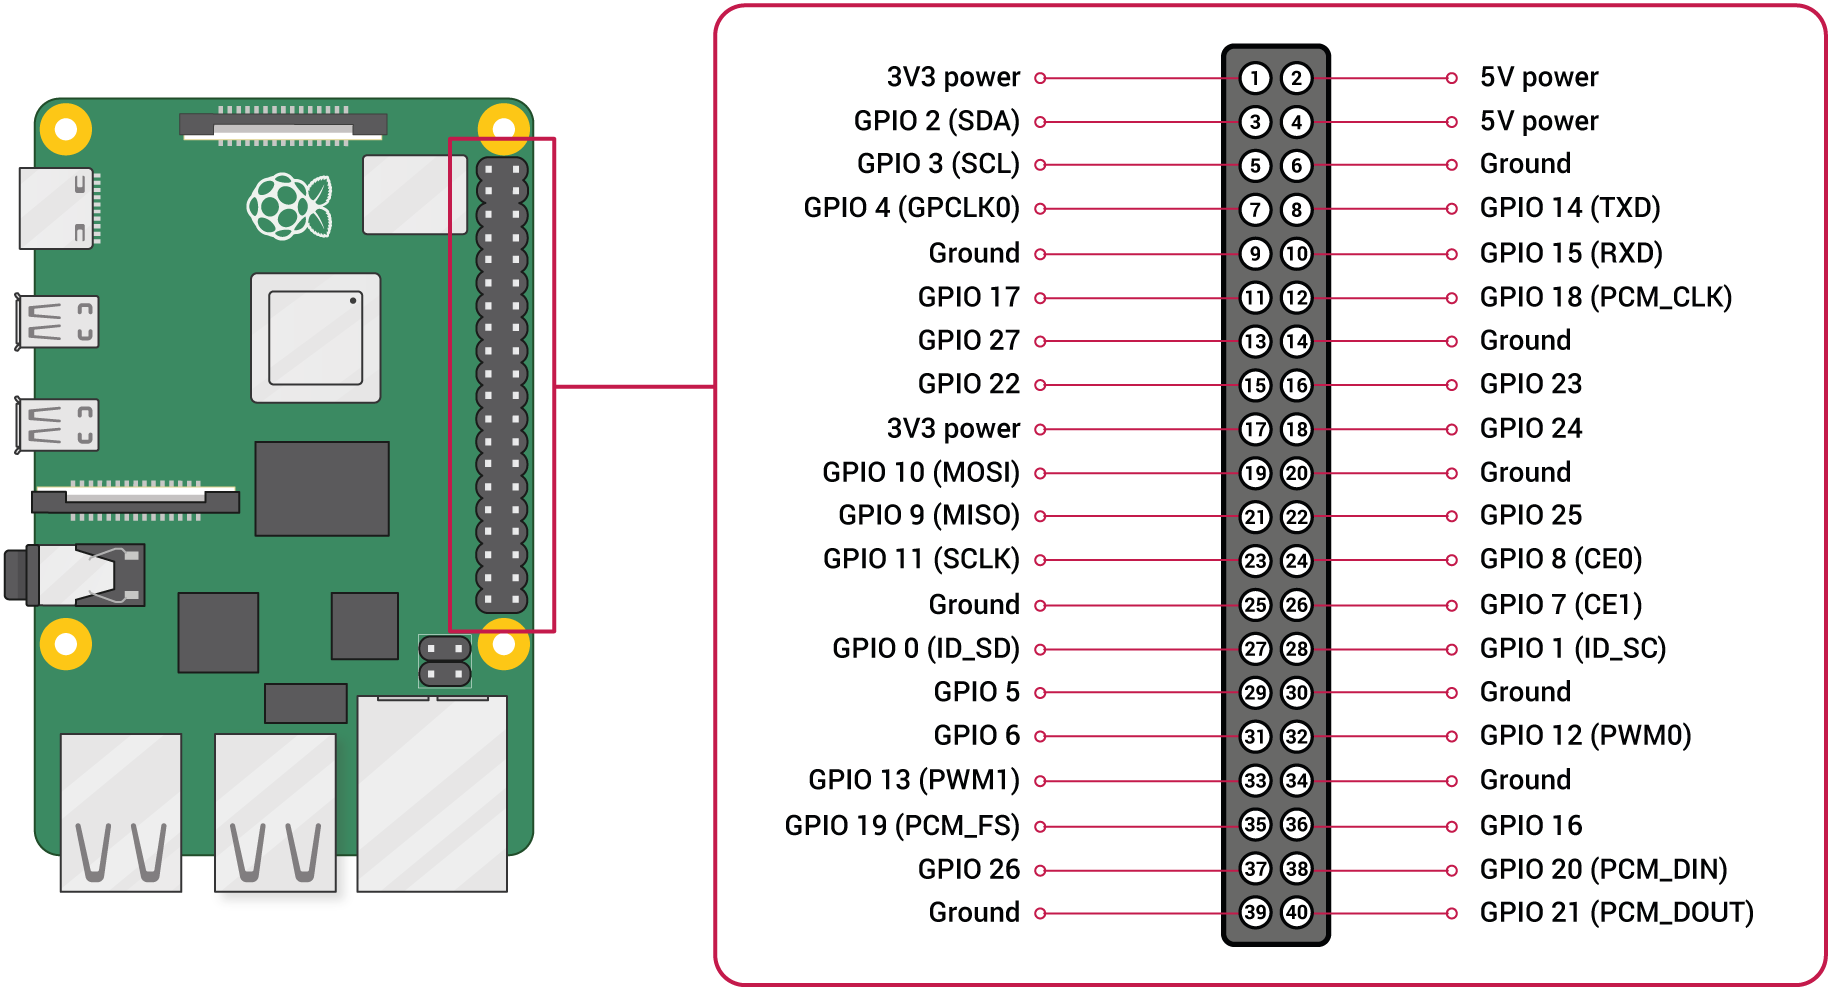
\includegraphics[width=\textwidth]{img/Rpi4_pin.png}
    \caption{Liste des PINs / GPIOs de la \glsentryname{raspberry}}
\end{figure}

\subsection{Branchements du servomoteur}

Pour le logiciel fournit, le servomoteur \gls{SG90} a des branchements spécifiques.
\begin{itemize}
    \item Fil marron : GND
    \item Fil rouge  : 5 V
    \item Fil orange : GPIO 12
\end{itemize}

\subsection{Branchements du panneau de LEDs}

En considérant que vous êtes dos au panneau :
\begin{itemize}
    \item Brancher la borne de droite du bornier à la broche GPIO 5
    \item La borne du milieu doit rester vide
    \item Brancher la borne de gauche du bornier au GND
\end{itemize}

\subsection{Branchements de la caméra}

La caméra \gls{RPiCamera} est fournie avec une nappe. Côté caméra :

\begin{enumerate}
    \item Ouvrer le connecteur d'accueil de nappe en tirant sur la languette
    \item Positionner la nappe de façon à ce que le trait de couleur bleu soit au dos de la lentille et fermer le
          connecteur. Faire de même sur le port d'accueil caméra de la \gls{raspberry}
    \item Positionner le trait bleu face au connecteur Ethernet.
\end{enumerate}
